\documentclass[aspectratio=169]{beamer}

% --- THEME & COLORS ---
% Metropolis is a modern, minimalist theme suitable for tech/research
\usetheme{metropolis}
\metroset{block=fill} % Fills blocks with color for better visibility
\metroset{progressbar=frametitle} % Adds a subtle progress bar to slides

% Custom Colors (Professional Dark Slate & Teal aesthetics)
\definecolor{TechDark}{RGB}{35, 37, 43}
\definecolor{TechAccent}{RGB}{0, 150, 136} % Teal for emphasis
\setbeamercolor{frametitle}{bg=TechDark, fg=white}
\setbeamercolor{alerted text}{fg=TechAccent}
\setbeamercolor{progress bar}{fg=TechAccent, bg=TechDark!50}

% --- PACKAGES ---
\usepackage{graphicx}
\graphicspath{{images/}}
\usepackage{booktabs}
\usepackage{tikz}
\usetikzlibrary{shapes.geometric, arrows, positioning}
\usepackage{caption}

% --- META DATA ---
\title{Datacenters vs Traditional HPC vs AI}
\subtitle{What makes AI computing so special?}
\author{Max Hawkins}
\date{}
\institute{Georgia Institute of Technology} % Inferred from context or placeholder

\begin{document}

% --- TITLE SLIDE ---
\maketitle

\begin{frame}{Overview}
    \begin{itemize}
        \item Traditional HPC: large-scale computing for scientific research
        \begin{itemize}
            \item Computational fluid dynamics or genome sequencing/assembly
            \item Large jobs, few users, long-running
        \end{itemize}
        \item Enterprise datacenters: computing, storage, and access for businesses
         \begin{itemize}
            \item Email, web browsing, cloud services
            \item Small jobs, many users, short-running
        \end{itemize}
        \item AI datacenters: large-scale computing for AI
        \begin{itemize}
            \item AI training and inference (e.g. LLMs, image generation, etc.)
            \item 'Large' jobs, many users, short/medium-running
        \end{itemize}
    \end{itemize}

\end{frame}

\begin{frame}{Caveat}
    \begin{center}
        These definitions and delineations are not clear-cut.\\[1ex]
        There is some overlap and convergence amongst these categories.
    \end{center}
\end{frame}

\begin{frame}{}
    \begin{center}
       \textbf{What task do you need to perform, \\and what does it take to do that?}
    \end{center}
\end{frame}


% --- SECTION 1 ---
\section{Traditional HPC}

\begin{frame}{What is Traditional HPC?}
    \begin{itemize}
        \item 'Large' scale systems (used to be the 'largest' synchronous computing scale)
        \item 'Supercomputers' - TOP500 list
        \item High-bandwidth, low-latency interconnects
        \item Shared filesystem
        \item Becoming dominated by GPU-based systems (exception: Fugaku)
    \begin{flushright}
        \begin{center}
            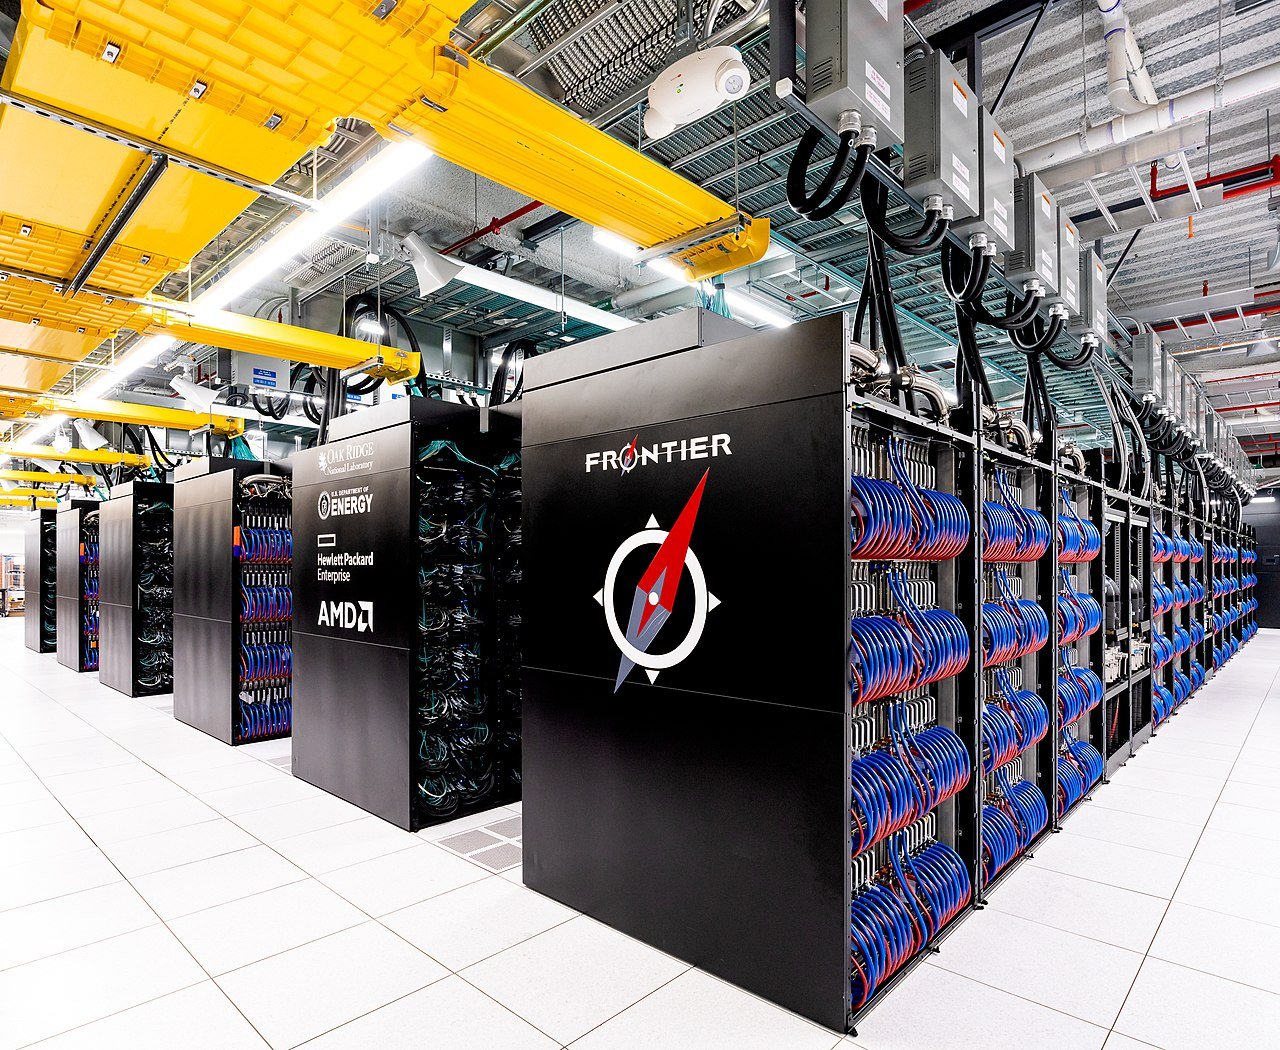
\includegraphics[width=0.45\textwidth]{images/frontier_internals.jpg}
        \end{center}
    \end{flushright}
    \end{itemize}
\end{frame}


\begin{frame}{Datacenters}
    \begin{itemize}
        \item 'Datacenters': What hosts our data, webservers, microservices, video streaming, etc.
        \item Smaller jobs - not much computing
        \item Emphasized reliability, scalability, latency,and cost-effectiveness
        \item CPU-dominated, but some HW-accelerated tasks (e.g. YouTube)
    \end{itemize}
\end{frame}

\begin{frame}{AI Datacenters}
    \begin{itemize}
        \item Throughput-focused: AI factories.
        \begin{itemize}
            \item "Tokens are commodities" - Jensen Huang (paraphrased)
        \end{itemize}
        \item Dominated by HW accelerators (GPUs, TPUs, etc.)
        \begin{itemize}
            \item Most AI models rely on matrix-matrix multiplications
        \end{itemize}
        \item Large jobs - Trillion-parameter AI models
        \item High-performance interconnects optimizing collective communication for training
        \item \textbf{DOMINATING} the computing market, supply chains, academic discussions, etc.

    \end{itemize}
\end{frame}

\begin{frame}{AI Datacenters}
    \begin{columns}[c]
        \column{0.5\textwidth}
            \begin{center}
                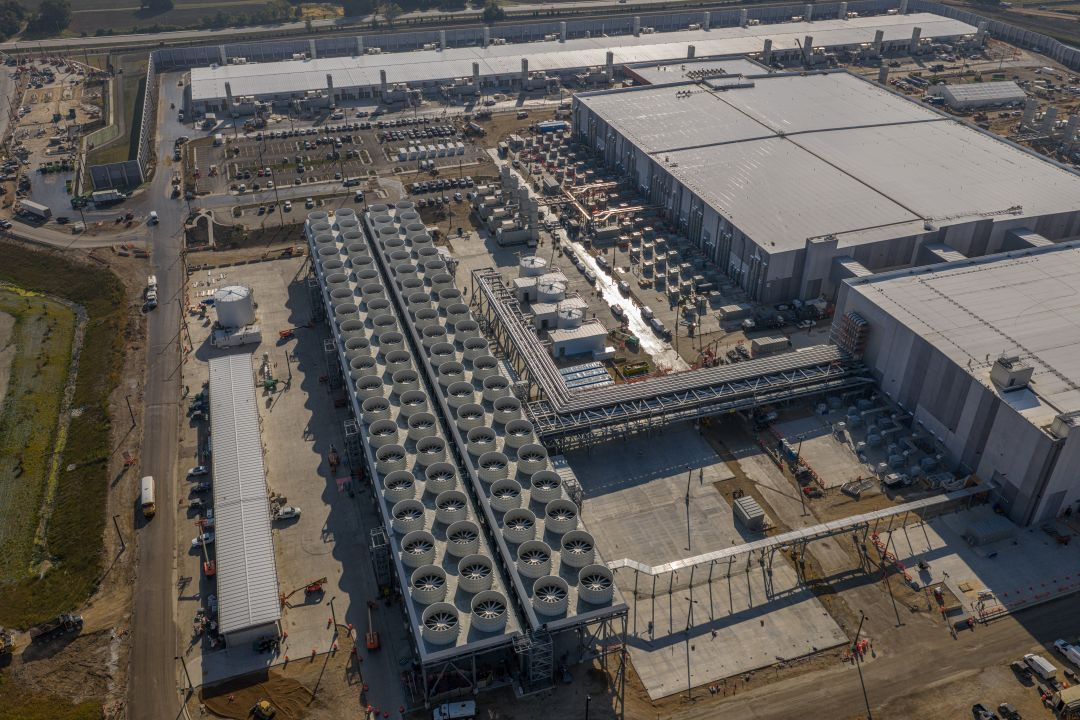
\includegraphics[width=\linewidth]{images/OMB-Image-1-Datacenter.jpg}
                Microsoft Fairwater \\
                (Hyperscale AI datacenter)
            \end{center}
        \column{0.5\textwidth}
            \begin{center}
                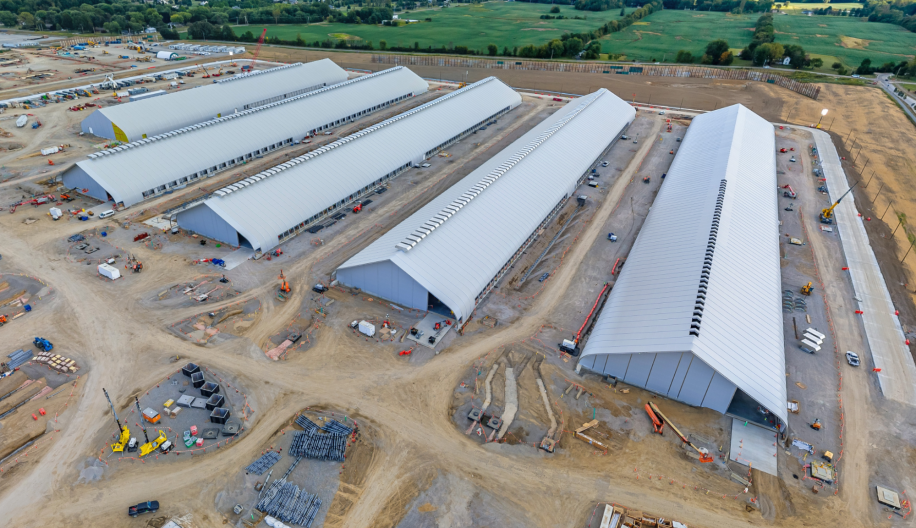
\includegraphics[width=\linewidth]{images/Meta-Promethesus-tent-construction.original.png}
                Meta's 'Rapid deployment structures' \\
                (Image source: DataCenterDynamics)
            \end{center}
    \end{columns}
\end{frame}

\begin{frame}{Density}
    \begin{itemize}
        \item Flop Density: *Exaflop/s* per rack! (MatMuls flip lots of transistors)
        \item Power Density: Approaching 1 MW per rack!
        \item Thermal Density: More power over slightly more space - More cooling required!
            \begin{itemize}
                \item Liquid cooling (now)
                \item Sub-ambient liquid cooling (future?)
            \end{itemize}
    \end{itemize}
\end{frame}

\begin{frame}{Reliability}
    When hardware fails or underperforms, what happens? What are the consequences?
    \begin{itemize}
        \item Datacenters: Degraded service or failover to backups
        \item HPC and AI: Jobs likely fail or slow to a crawl
        \item AI Training: The scale is so large, failure is always imminent.
        \begin{itemize}
            \item Meta's Llama 3 paper - good section on this
            \item Straggler (underperforming) nodes have a large impact
            \item How much to checkpoint vs accept loss of progress?
        \end{itemize}
    \end{itemize}
\end{frame}

\begin{frame}{Market Share}
    HPC used to dominate the high-performance computing market.\\
    \textit{Not anymore.}\\

    \begin{center}
        \textbf{\Large "HPC is a rounding error in the era of AI"}
    \end{center}
\end{frame}

\end{document}
